\setlength{\columnsep}{3pt}
\begin{flushleft}

\bigskip
\paragraph{Server}
\begin{itemize}
	\item Server is a computer system that provides a specific service 24x7.
\end{itemize}

\paragraph{Client}
\begin{itemize}
	\item Client is a computer system that accesses a specific service from a server.
\end{itemize}

For eg: 
\begin{itemize}
	\item When you connect to youtube, your system becomes client to youtube server.
	\item When you connect to facebook, your system becomes client to facebook server.
	\item When you connect to database, your system becomes client to Database server.
\end{itemize}

	\begin{figure}[h!]
	\centering
	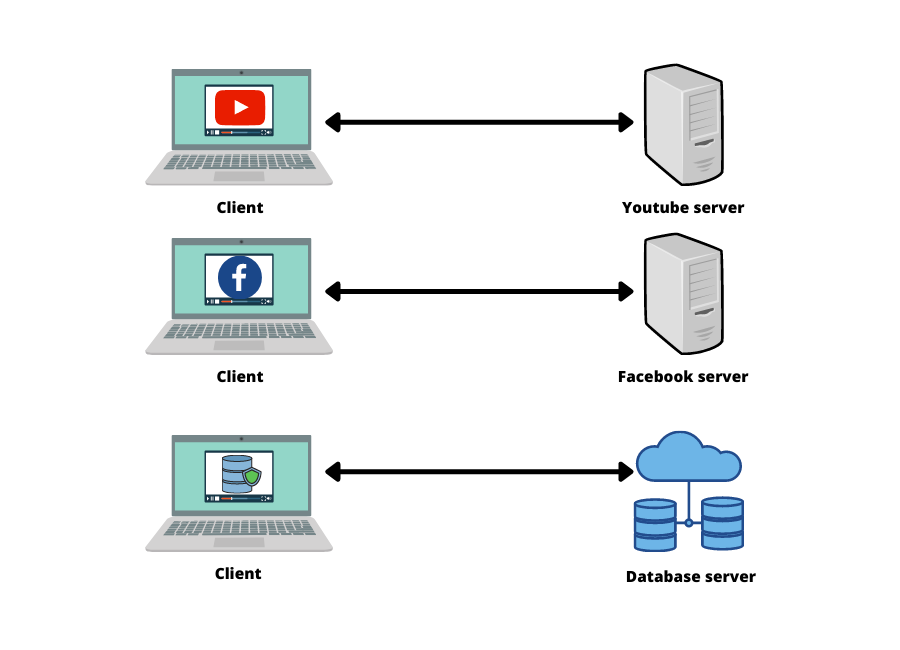
\includegraphics[scale=.5]{content/chapter19/images/server-client.png}
	\caption{Server \& client}
	\label{fig:ssh_server_client}
\end{figure}


\end{flushleft}
\newpage


